\chapter{Specific cases of fluid flow - Cylindrical}
\label{ch:momcasescyl}

\section{Flow through a pipe}

\begin{figure}[h]
\begin{center}
\framebox{
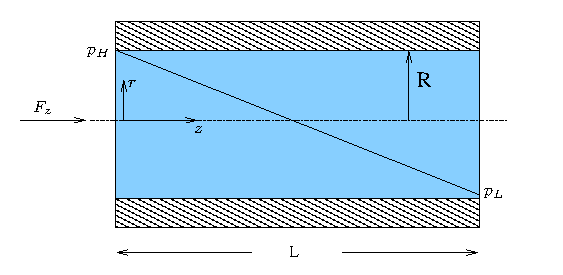
\includegraphics[scale=1.0]{images/c12-pipeflowfig.ps}
 }
\end{center}
\caption{Pipe Flow}
\label{pipeflow}
\end{figure}

Figure \ref{pipeflow} shows the problem definition.


Assumptions:
\begin{itemize}
\item Flow is unidirectional: Only $u_z$ is to be known, $u_r$ and $u_\theta$ are zero
\item Flow is steady state: $\frac{\partial u_z}{\partial t} = 0$
\item Flow is fully developed: $\frac{\partial u_z}{\partial z} = 0$
\item Pressure gradient is constant: $\frac{\partial p}{\partial z} = \frac{\Delta p}{L}$
\end{itemize}


Boundary Conditions:
\begin{itemize}
\item No slip condition at pipe wall: at $r=R$, $u_z=0$.
\item Finite velocity at center: at $r=0$, $u_z \ne \infty$.
\end{itemize}


Use N-S equation in cylindrical co-ordinate system for $u_z$ and eliminate terms as per the assumptions above.

\begin{align}
\frac{\partial u_z}{\partial t} + u_r \frac{\partial u_z}{\partial r} + \frac{u_\theta}{r} \frac{\partial u_z}{\partial \theta} + u_z \frac{\partial u_z}{\partial z} = F_z-\frac{1}{\rho}\frac{\partial p}{\partial z} \nonumber \\
+ \nu \left[ \frac{1}{r} \frac{\partial}{\partial r}\left( r \frac{\partial u_z}{\partial r} \right) + \frac{1}{r^2}\frac{\partial^2 u_z}{\partial \theta^2} + \frac{\partial^2 u_z}{\partial z^2} \right] 
\end{align}

\begin{equation*}
0 = F_z-\frac{1}{\rho}\frac{\Delta p}{L} + \frac{\mu}{\rho} \frac{1}{r} \frac{\partial}{\partial r}\left( r \frac{\partial u_z}{\partial r} \right)  
\end{equation*}

\begin{equation*}
u_z  = -\left[ \frac{\rho F_z}{4 \mu}-\frac{1}{4\mu}\frac{\Delta p}{L} \right] r^2 + C_1 \ln(r) + C_2
\end{equation*}

Using boundary conditions,
$$C_1 = 0$$
\begin{equation*}
C_2  = \left[ \frac{\rho F_z}{4 \mu}-\frac{1}{4\mu}\frac{\Delta p}{L} \right] R^2 
\end{equation*}

\begin{equation*}
u_z = \left[ \frac{\rho F_z}{4 \mu}-\frac{1}{4\mu}\frac{\Delta p}{L} \right] (R^2 - r^2)
\end{equation*}

Using Newton's law $$\sigma_{21} = \tau_{zr} = \mu \frac{\partial u_z}{\partial r}$$

$$\tau_{zr} = \left[ \frac{\rho F_z}{4 \mu}-\frac{1}{4\mu}\frac{\Delta p}{L} \right] (-2r) $$

The solution is plotted schematically in figure \ref{pfslfg}.

\begin{equation*}
u_z|_{max} = \left[ \frac{\rho F_z}{4 \mu}-\frac{1}{4\mu}\frac{\Delta p}{L} \right] R^2
\end{equation*}

Average flow velocity $\bar{u}_z$:
$$ \bar{u}_z = \frac{\int_0^R{u_z 2\pi r dr}}{\int_0^R{2\pi r dr}} = \frac{1}{2} u_z|_{max}$$
Volume flow rate $\dot{V}$:
$$ \dot{V} = \pi r^2 \bar{u}_z = \left[ \frac{\rho F_z}{8 \mu}-\frac{1}{8\mu}\frac{\Delta p}{L} \right] \pi R^4 $$

Mass flow rate $\dot{M}$ (Hagen-Poiseuille Equation):
$$ \boxed{\dot{M} = \rho \dot{V} = \left[ \frac{\rho^2 F_z}{8 \mu}-\frac{\rho}{8\mu}\frac{\Delta p}{L} \right] \pi R^4} $$

\begin{figure}[h]
\begin{center}
\framebox{
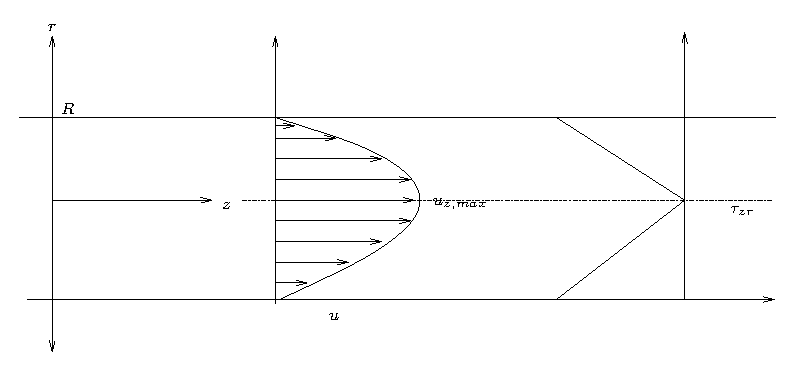
\includegraphics[scale=1.0]{images/c12-pipeflowsolfig.ps}
}
\end{center}
\caption{Solution to Pipe Flow}
\label{pfslfg}
\end{figure}

% --------------------------------------------------------------------
\begin{figure}[h]
\label{axialfilmflow}
\begin{center}
\frame{
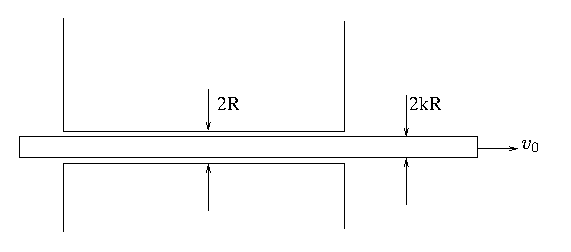
\includegraphics[scale=1.0]{images/c12-filmflowfig.ps}
}
\end{center}
\caption{Axial film flow}
\end{figure}

\begin{question}
Axial film flow: Problem 2B.7 of~\cite{bls}. A cylindrical rod of radius $kR$ moves axially with velocity $v=v_0$ along the axis of a cylindrical cavity of radius $R$ as shown in figure below. Assuming that the pressure at both ends of the cavity is same and fluid flows through the annular region only because of the rod motion. (a) Find the velocity distribution in the narrow annular region. (b) Find the mass flow rate through the annular region. (c) Obtain the viscous force acting on the rod over a length L.\\
\end{question}
\begin{solution}[print]
(a) $$ {u_z \over u_0} = { \ln \left( r / R \right) \over \ln k} $$
(b) $$ \dot{M} = {\pi R^2 u_0 \rho \over 2} \left( {1 - k^2 \over \ln \left(1 /k\right)} - 2 k^2 \right)$$
(c) $$ F_z = {2 \pi L \mu u_0 \over \ln \left( 1 / k \right)} $$
\end{solution}

% --------------------------------------------------------------------

\begin{figure}[h]
\begin{center}
\frame{
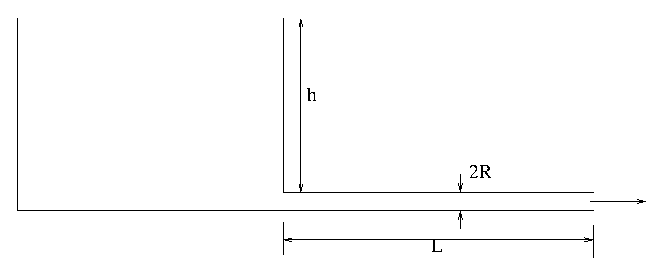
\includegraphics{images/c12-LeakingTank.eps}
}
\end{center}
\caption{Leaking Tank}
\label{LeakingTank}
\end{figure}

\begin{question}
Leaking tank: Water of viscosity $\mu$ = \SI{0.01}{\pascal\second} and density $\rho$ = \SI{1000}{\kilo\gram\per\metre\cubed} from a large tank is to be transported using a rigid smooth tube of \SI{1}{\centi\metre} dia connected at the bottom across a distance of $L$ = \SI{100}{\metre} as shown in figure~\ref{LeakingTank}. Assuming that at steady state the tank is large enough that the height of water in it ($h$) does not change much in time, what should be $h$ such that the flow rate in the tube is one litre per minute. 
\end{question}
\begin{solution}[print]
\end{solution}

% --------------------------------------------------------------------
\begin{figure}[h]
\begin{center}
\resizebox{5in}{!}{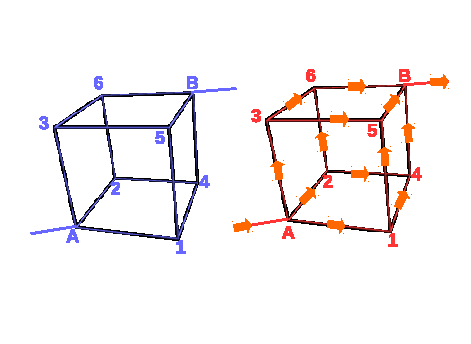
\includegraphics[bb=0 0 210 149, clip]{images/c12-CubicPipeNetwork2.eps}}
\end{center}
\caption{Cubic network of pipes}
\label{CubicPipeNetwork}
\end{figure}

\begin{question}
Cubic network of pipes: Problem 2B.12 of~\cite{bls}. A fluid is flowing in laminar flow from A to B through a network of tubes, as depicted in figure~\ref{CubicPipeNetwork}. Obtain an expression for the mass flow rate $w$ of the fluid entering at A (or leaving at B) as a function of the modified pressure drop $p_A - p_B$. Neglect the disturbances at the various tube junctions. Neglect any body forces that may act on some of the segments due to their orientation.\\
\end{question}
\begin{solution}[print]
Writing volume flow rate through each pipe at junctions as follows:

At junction 2:
$$ V_{A2} = V_{26} + V_{24}$$
	$${p_2 - p_A \over L} D^4 { \pi \over 8 \mu} = {p_6 - p_2 \over L} D^4 {\pi \over 8 \mu}  + {p_4 - p_2 \over L} D^4 {\pi \over 8 \mu} $$
$$ p_A = 3 p_2 -p_4 -p_6 $$

Skip the term $ {D^4 \pi \over L 8 \mu}$ for the remaining equations.

At junction 3:
$$ V_{A3} = V_{36} + V_{35}$$
$$ \left( p_3 - p_A \right) = \left( p_6 - p_3 \right) + \left( p_5 - p_3 \right) $$
$$ p_A = 3 p_3 -p_5 -p_6 $$

At junction 6:
$$ V_{36} + V_{26} = V_{6B}$$
$${p_6 - p_3 \over L} D^4 + {p_6 - p_2 \over L} D^4 = {p_B - p_6 \over L} D^4 $$
$$ p_B = 3 p_6 -p_2 -p_3 $$

Add the above three to obtain:

$$ 3p_B = 3 \left( p_4 + p_5 + p_6 \right) - 2 \left( p_1 + p_2 + p_3\right)$$

At junction 5:
$$ V_{35} + V_{15} = V_{5B}$$
$${p_5 - p_3 \over L} D^4 + {p_5 - p_1 \over L} D^4 = {p_B - p_5 \over L} D^4 $$
$$ p_B = 3 p_5 -p_3 -p_1 $$

At junction 1:
$$ V_{A1} = V_{15} + V_{14}$$
$${p_1 - p_A \over L} D^4 = {p_5 - p_1 \over L} D^4 + {p_4 - p_1 \over L} D^4 $$
$$ p_A = 3 p_1 -p_4 -p_5 $$


At junction 4:
$$ V_{14} + V_{24} = V_{4B}$$
$${p_4 - p_1 \over L} D^4 + {p_4 - p_2 \over L} D^4 = {p_B - p_4 \over L} D^4 $$
$$ p_B = 3 p_4 -p_1 -p_2 $$

Add the above three to obtain:

$$ 3p_A = 3 \left( p_1 + p_2 + p_3 \right) - 2 \left( p_4 + p_5 + p_6\right)$$

Write the flow rate at junction A:
$$ V_A = V_{A1} + V_{A2} + V_{A3}$$
$$ V_A = \left( p_1 - p_A + p_2 - p_A + p_3 - p_A \right) {D^4 \over L} { \pi \over 8 \mu} $$
$$ V_A = \left( p_1 + p_2 + p_3 - 3 p_A \right) {D^4 \over L} { \pi \over 8 \mu} $$

Multiply the equations with 2 and 3 to add to eliminate $ p_4 + p_5 + p_6$ term and give:

$$ 6 p_B + 9 p_A = 6 \left( p_4 + p_5 + p_6 \right) - 4 \left( p_1 + p_2 + p_3 \right) + 9 \left( p_1 + p_2 + p_3 \right) - 6 \left( p_4 + p_5 + p_6 \right)$$
$$ 6 p_B + 9 p_A = 5 \left( p_1 + p_2 + p_3 \right) $$

Now, using the equation for $V_A$, we can write:

$$ V_A = \left({ { 6p_B + 9 p_A} \over 5} - 3 p_A \right) {D^4 \over L} { \pi \over 8 \mu} $$
$$ V_A = {6 \pi \over 40 \mu} \left( p_B - p_A \right) {D^4 \over L} $$
$$ V_A = {3 \pi \over 20 \mu} \left( p_B - p_A \right) {D^4 \over L} $$

$$\dot{M} = {3 \pi \left( p_A - p_B \right) R^4 \rho \over 20 \mu L}$$
\end{solution}

% --------------------------------------------------------------------

\begin{question}
Blasius equation: Section 4.1 of~\cite{gaskell}. For steady viscous flow through a circular tube, the axial velocity profile is given approximately by the Blasius' equation below.
$$ u = u_0 \left( 1 - {r \over R} \right)^m$$
For turbulent flow, $m = {1 / 7}$. Assuming the density is constant, what is the average velocity? Is it closer to the maximum than in the case of Poiseuille flow? Comment.\\
\end{question}
\begin{solution}[print]
$0.817 u_0$
\end{solution}

% --------------------------------------------------------------------
\begin{figure}[h]
\begin{center}
\frame{
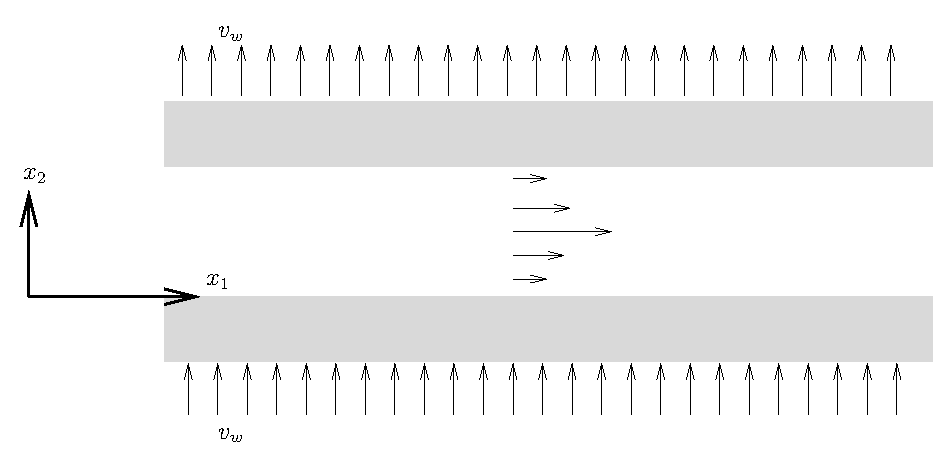
\includegraphics[scale=1.0]{images/c12-porouschannelfig.ps}
}
\end{center}
\caption{Channel flow between porous walls}
\label{PorousChannel}
\end{figure}

\begin{question}
Channel flow between porous walls: Problem 3B.16 of~\cite{bls}. Newtonian fluid flows through a rectangular channel with porous walls with a height $h$ and infinite extensions along $x_1$ and $x_3$ directions as shown in figure~\ref{PorousChannel}. The fluid leaks through the walls at a constant velocity of $v_w$. The plane flow is steady, density $\rho$ and viscosity $\mu$ are constant and there are no body forces. The flow takes place due to a constant pressure gradient $\Delta p \over L$. Velocity is fully developed along $x_1$. (a) Use the continuity equation to obtain $u_2(x_2)$. (b) Write the Navier-Stokes equation for $u_1$ after simplification. (c) Assuming no slip boundary conditions applicable for $u_1$, show that the velocity distribution can be given by the expression below.
 (d) Show that in the limit $v_w \rightarrow 0$, we retrieve the velocity profile of a plane channel flow. Note the location of axes different from the ones used in the class.
$$u_1(x_2) = {\Delta p \over L} {h \over \rho v_w} \left( {x_2 \over h} - {{1- e^{v_w x_2 \over \nu}} \over {1 - e^{v_w h \over \nu}}} \right)$$
\end{question}
\begin{solution}[print]
\end{solution}

% --------------------------------------------------------------------

\begin{question}
Euler equation: Euler equation governs the flow of inviscid fluids i.e., fluids with nearly zero viscosity. (a) Use the information given at the end of the question paper and write down Euler equation in one dimension case for flow in a vertical tube due to both gravity as well as pressure gradient. (b) Show that in steady state, it reduces to the following expression popularly known as Bernouli equation.
$$ \frac{p}{\rho} + gz + \frac{v_z^2}{2} = \text{constant}$$
\end{question}
\begin{solution}[print]
\end{solution}

% --------------------------------------------------------------------

\begin{question}
Couette flow: The Navier-Stokes equation for the $\theta$ component of velocity in cylindrical coordinate system is given to you. Annular region between two coaxial cylindrical surfaces of radii $r_i$ and $r_o$ (for inner and outer radii, respectively) is filled with a fluid. The outer cylinder is rotating with an angular velocity of $\Omega_o$ and the inner cylinder is rotating with an angular velocity of $\Omega_i$, both clockwise. Assume that the fluid flow is uniform, steady state and fully developed and is only due to the rotation of outer cylinder. (a) Determine the velocity distribution in the liquid in the annular region. (b) Show that the result will approximate to Newton's Law when the difference of radii is very small compared to either radii.
\end{question}
\begin{solution}[print]
\end{solution}

% --------------------------------------------------------------------

\begin{question}
Channel flow of two stratified immiscible fluids: Section 2.5 of~\cite{bls}. Two immiscible incompressible fluids of viscosities $\mu_1$ (bottom) and $\mu_2$ (top) are flowing between two stationary parallel plates under a pressure gradient $\Delta P \over L$. Assume $\mu_1 > \mu_2$. The thickness of the two layers $\delta$ is same. (a) Derive an expression for the shear stress as a function of distance between the two plates. (b) Determine the location of zero shear stress from the bottom. (c) Draw schematically the shear stress profile.
\end{question}
\begin{solution}[print]
\end{solution}

% --------------------------------------------------------------------

\begin{question}

The Navier-Stokes equation for the $\theta$ component of velocity in cylindrical coordinate system is given below. Annular region between two coaxial cylindrical surfaces of radii $r_i$ and $r_o$ (for inner and outer radii, respectively) is filled with a fluid. The outer cylinder is rotating with an angular velocity of $\Omega_o$ and the inner cylinder is rotating with an angular velocity of $\Omega_i$, both clockwise. Assume that the fluid flow is uniform, steady state and fully developed and is only due to the rotation of outer cylinder. (a) Determine the velocity distribution in the liquid in the annular region. (b) Show that the result will approximate to Newton's Law when the difference of radii is very small compared to either radii.

$$\frac{\partial v_\theta}{\partial t} + v_r \frac{\partial v_\theta}{\partial r} + \frac{v_\theta}{r} \frac{\partial v_\theta}{\partial \theta} + \frac{v_r v_\theta}{r} + v_z \frac{\partial v_\theta}{\partial z} = $$
$$ F_\theta -\frac{1}{\rho r}\frac{\partial p}{\partial \theta} \nonumber + \nu \left[ \frac{\partial}{\partial r}\left(\frac{1}{r} \frac{\partial \left\{rv_\theta\right\}}{\partial r} \right) + \frac{1}{r^2}\frac{\partial^2 v_\theta}{\partial \theta^2} + \frac{2}{r^2}\frac{\partial v_r}{\partial \theta} + \frac{\partial^2 v_\theta}{\partial z^2} \right] $$

\end{question}

\begin{solution}[print]

With the assumptions of steady state, fully developed uniform flow without any body forces or pressure gradients, set $\partial v_\theta \over \partial t$, $v_r$, $v_z$, $\partial v_\theta \over \partial \theta$, $F_\theta$ and $\partial p \over \partial \theta$ and variations along $z$ to zero.

$$\frac{\partial}{\partial r}\left(\frac{1}{r} \frac{\partial \left\{rv_\theta\right\}}{\partial r} \right) = 0 $$

Integrating twice and recognizing that the first integration constant $C_1$ anyway needs to be found out (so that we can drop the 2 in the denominator),

$$ v_\theta = C_1 r + {C_2 \over r}$$

Using the boundary conditions of $v_\theta = r_i \Omega_i$ at $r = r_i$ and $v_\theta = r_o \Omega_o$ at $r = r_o$,

$$r_i \Omega_i = C_1 r_i + {C_2 \over r_i}$$
$$r_o \Omega_o = C_1 r_o + {C_2 \over r_o}$$

Multiplying the first equation with $r_i$ and the second with $r_o$ and substracting,

$$C_1 = { r_i^2 \Omega_i - r_o^2\Omega_o \over r_i^2 - r_o^2} $$

Similarly, divide the first equation with $r_i$ and the second with $r_o$ and substract to get,

$$C_2 = {(\Omega_i-\Omega_o) r_i^2 r_o^2 \over r_o^2 - r_i^2}$$

Substituting,

$$\boxed{
v_\theta = { r_i^2 \Omega_i - r_o^2\Omega_o \over r_i^2 - r_o^2} r + {(\Omega_i-\Omega_o) r_i^2 r_o^2 \over r_o^2 - r_i^2} {1 \over r}
} $$

To approximate the situation to that of Newton's law, set $\Omega_i=0$, $r_o\Omega_o = u_o$, $r_i = R \approx r_o$, $r_o - r_i = \delta$, $r = R + y$.

$$ v_\theta = { - r_o u_o \over r_i^2 - r_o^2} r + {-u_o r_i^2 r_o \over r_o^2 - r_i^2} {1 \over r} $$

$$ v_\theta = { R u_o \over 2R\delta} \left({ r^2 - R^2 \over r}\right) $$

$$ v_\theta 
= { u_o \over 2\delta} \left({ (r +  R) y \over r}\right) 
= { u_o y \over \delta} \left[{ r +  R \over 2 r}\right] 
$$

In the limit of $y$ being very small compared to $R$, the term in the square brackets tends to unity, leaving the relation

$$ \boxed{ v_\theta = { u_o y \over \delta} }$$

which is the same as definition of Newton's law.
\end{solution}

% --------------------------------------------------------------------
